\subsection{Синтез речи}
\subsubsection{Введение}
Синтез речи из текста (text--to--speech, TTS синтез) предоставляет дополнительные возможности по улучшению устной речи для людей, изучающих иностранный язык. Так, доступ к эталонному произношению в аудио формате для произвольного фрагмента текста позволяет студенту ознакомиться с особенностями иностранной речи на слух и служить примером при обучении.

Создание речи по тексту является сложной задачей в области алгоритмов машинного обучения несмотря на многие годы исследований\cite{taylor2009text}. С течением времени несколько раз сменялись лидирующие технологии в этой области. На протяжении длительного времени метод конкатенации мелких фрагментов заранее записанной речи\cite{hunt1996unit} являлся предпочтительным. Следующим шагом в развитии TTS--синтеза был подход генерации непрерывной последовательности параметров речи с использованием скрытых марковских моделей\cite{tokuda2000speech}, который решил проблемы с помехами, возникающими на стыках звуков в предыдущем методе. Тем не менее, речь, созданная этими системами звучит искусственно в сравнении с живой человеческой речью.

Модель WaveNet\cite{oord2016wavenet}, позволяет создавать высокореалистичные аудио фрагменты, довольно хорошо приближенные к человеческой речи. Однако входные данные для реализации такой сети требуют высокого уровня знаний в лингвистике целевого языка.

Архитектура Tacotron, основанная на sequence--to--sequence трансформации упрощает стандартный процесс синтеза речи путем замены ручного создания лингвистических признаков на специально обученную нейронную сеть.

Одним из последних достижений в области синтеза речи является архитектура Tacotron 2\cite{shen2018natural}, сочетающая в себе преимущества всех предыдущих подходов: sequence--to--sequence модель для генерации мел--спектро\-грамм, похожая на Tacotron, и вокодер, основанный на WaveNet. Данная модель показывает результаты, крайне близкие к живой человеческой речи, одновременно сокращая размеры модели WaveNet.

В последующих пунктах эти подходы будут рассмотрены подробнее.

\subsubsection{Синтез речи с помощью модели WaveNet}
\label{section:wavenet}
Ключевая идея WaveNet --- генерирование звуковых волн с использованием идей PixelRNN \cite{van2016pixel} и PixelCNN\cite{oord2016conditional} сетей. На протяжении долгого времени моделирование <<сырых>> звуковых волн избегалось ввиду больших объемов данных и связанных с этим сложностей. Так, одна секунда речи содержит около 16,000 точек, которые нужно смоделировать. Построение модели, которая предсказывает каждую следующую точку с учетом всех предыдущих --- весьма нетривиальная задача.

Двухмерные подходы, представленные в PixelRNN и PixelCNN моделях, демонстрируют высокие результаты в задачах моделирования/восстановления изображений, где им необходимо воссоздавать тысячи пикселей. Одномерная сеть WaveNet заимствует концепции этих моделей.

Совместная вероятность звуковой волны $\mathbf{x} = \{x_1, \dots, x_T\}$ может быть выражена в виде равенства
$$P(\mathbf{x}) = \prod_{t = 1}^{T} P(x_t | x_1, \dots, x_{t - 1}).$$

Таким образом на каждый фрагмент $x_t$ влияют все предыдущие.

Вероятностное распределение моделируется с помощью сверточной сети, структура которой представлена на рисунке \ref{dilated-cnn}. Модель не содержит pooling--слоев и размерность вывода совпадает со входной размерностью.

\begin{figure}[h]
	\centering
	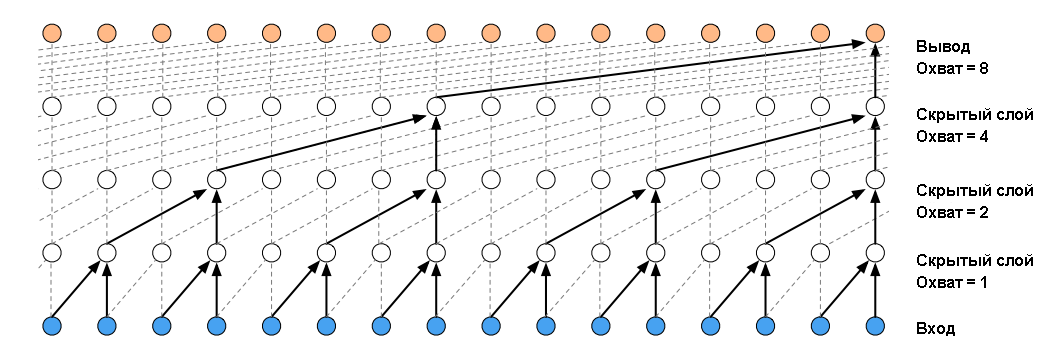
\includegraphics[width=0.7\textwidth]{dilated-cnn}
	\caption{Визуальное представление расширяемой сверточной сети.}
	\label{fig:dilated-cnn}
\end{figure}

Одна из ключевых особенностей сети такой структуры --- применение фильтра свертки по большему полю, чем размер фильтра путем пропуска узлов с некоторым шагом. Еще одним важным свойством сети является то, что каждое выходное значение может зависеть только от входных параметров на предыдущих отрезках времени, т.е. не может зависеть от будущего.

Сеть обучается на звуковых волнах записей не синтезированной человеческой речи. После обучения сеть может генерировать новые звуковые волны, шаг за шагом. На каждом шаге значение берется из вероятностного распределения, которое выдает WaveNet. На следующем этапе это значение подается на вход сети, после чего создается новая точка. Такой пошаговый подход необходим для создания сложных и реалистичных звуковых фрагментов.

Однако для синтеза речи по тексту этого ещё недостаточно. Помимо данных, полученных на предыдущих этапах будем подавать на вход сети дополнительный вектор $\mathbf{h}$, выступающий в качестве условия:
$$P(\mathbf{x} | \mathbf{h}) = \prod_{t = 1}^{T} P(x_t | x_1, \dots, x_{t - 1}, \mathbf{h}).$$

Введение условия позволяет управлять голосом, которым произносится речь. А главное, при помощи вектора условия мы можем задать, что именно должна произносить модель. Необходимо трансформировать текст в последовательность лингвистических и фонетических признаков, которые содержат информацию о текущей фонеме, слоге, слове, и так далее, после чего подать эту информацию в качестве условия. Таким образом вывод сети будет обусловлен не только предыдущими результатами, но и текстом, который необходимо произнести. В противном случае модель будет генерировать бессмысленные фрагменты, хоть и похожие на человеческую речь.

Рассмотренная здесь глубокая генеративная нейронная сеть WaveNet позволяет напрямую генерировать звуковые волны. Данный класс сетей зависит от предыдущих значений и использует специальный вариант сверточных фильтров, поле зрения которых экспоненциально растет с глубиной сети. Такие отличительные особенности позволяют моделировать длительные временные зависимости в аудио сигнале, синтезировать реалистичную речь и избавиться от недостатков предыдущих подходов. В следующем пункте будет рассмотрено дальнейшее развитие сетей WaveNet в виде архитектуры Tacotron.

\subsubsection{Архитектура Tacotron 2 для синтеза речи}
Архитектура нейронных сетей Tacotron 2 была разработана Google совместно с University of California, Berkeley в 2017 году\cite{shen2018natural}. Система состоит из рекуррентной sequence--to--sequence сети, которая переводит текст в мел--спектрограммы, и модифицированной моделью WaveNet, которая используется в качестве вокодера\footnote{Вокодер --- устройство для анализа и синтеза голоса на основе произвольного сигнала. Может использоваться для сжатия, шифрования и трансформации аудио данных.}, синтезируя звуковые волны. Общая структура системы изображена на рисунке \ref{fig:tacotron-architecture}.

\begin{figure}[h]
	\centering
	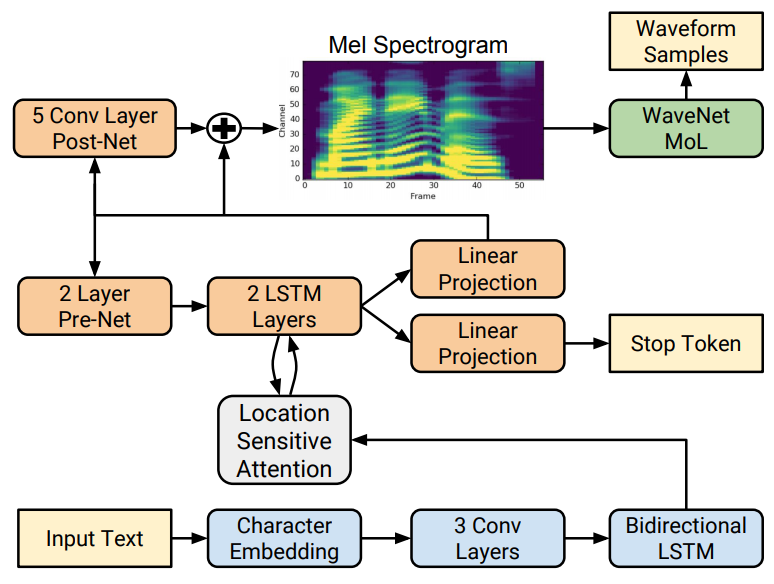
\includegraphics[width=0.7\textwidth]{tacotron-architecture}
	\caption{Структура системы Tacotron 2.}
	\label{fig:tacotron-architecture}
\end{figure}

Промежуточное представление звуковых данных в виде мел--спектрограммы позволяет поддерживать модульную структуру системы и обучать два компонента --- сеть, генерирующую спектрограмму и WaveNet по отдельности.

Сеть генерации спектрограмм имеет архитектуру sequence--to--sequence и состоит из энкодера и декодера, а также механизма внимания. Энкодер представляет собой двунаправленную LSTM сеть\cite{huang2015bidirectional}, которая переводит входные данные во внутреннее представление --- вектор признаков. Далее к вектору признаков применяется механизм внимания с функцией внимания из \cite{chorowski2015attention}:
$$\operatorname{Attention}(\mathbf{q}_{t - 1}, \mathbf{h}_t) = \alpha_t = \operatorname{Softmax}(\mathbf{w}^\top \tanh (W\mathbf{q}_{t - 1} + V\mathbf{h}_t + Uf_t + \mathbf{b})),$$
$$f_t = F \ast \alpha_{t - 1}.$$
Здесь $\mathbf{q}_t$ --- состояние сети декодера в момент времени $t$, $\mathbf{h}_t$ --- состояние сети энкодера в момент времени $t$, $\alpha_t$ --- вектор весов внимания в момент времени $t$, векторы $\mathbf{w}, \mathbf{b}$ и матрицы $W, V, U$ подбираются в процессе обучения, $F$ --- матрица свертки.

Декодер --- это рекуррентная однонаправленная LSTM сеть, зависящая от своих предыдущих значений, которая моделирует мел--спектрограмму по вектору признаков, полученному из механизма внимания и сети--энкодера.

К этой базовой структуре из декодера, энкодера и механизма внимания, который мы уже рассматривали в пункте \ref{section:e2e-approach}, добавлено несколько модификаций:
\begin{itemize}
	\item Прежде чем результат предыдущего шага подается на вход декодеру, он проходит через небольшую сеть из 2 полносвязных слоев с функцией активации ReLU. Такая модификация необходима при обучении механизма внимания.
	\item Результат работы декодера проходит через линейное преобразование и 5--слойную CNN сеть с фильтрами $5 \times 1$ с функциями активации $\tanh$. Эта небольшая сеть пост--обработки направлена на общее повышение качества генерируемого спектра.
	\item Для определения вероятности конца последовательности вывод декодера и контекст внимания преобразуются в скаляр и проходят через $\sigma$--функцию активации. Процесс генерации останавливается, если эта вероятность превышает $0.5$.
	\item Для регуляризации сверточных сетей в системе используются dropout слои с вероятностью 0.5, а для LSTM эта вероятность составляет 0.1.
\end{itemize}

Конечный результат в виде звуковых волн генерируется при помощи модифицированной WaveNet сети, описанной предыдущем пункте \ref{section:wavenet}. Мел--спектрограммы, полученные в предыдущем компоненте подаются на вход WaveNet сети в качестве условия. Модификации заключаются в улучшениях производительности и архитектуры, заимствованных из PixelCNN++ сетей \cite{salimans2017pixelcnn++} и Parallel WaveNet \cite{oord2018parallel}.

\subsubsection{Вывод по главе}
В этой главе мы проанализировали возможности применения синтеза речи с помощью алгоритмов машинного обучения в контексте изучения иностранных языков. Были рассмотрены лидирующие на данный момент подходы в этой области: глубокие нейронные сети WaveNet и основанная на них архитектура Tacotron. Синтез речи прошел через годы эволюции, за которые были предложены и опробованы разнообразные подходы. Одно из наиболее прогрессивных решений, Tacotron 2, позволяет синтезировать речь высокого качества, практически не отличимую от человеческой, а обучение можно производить на сырых данных, не требующих сложной подготовки в виде ручной идентификации признаков и анализа особенностей конкретного языка. Использование технологии синтеза речи в мобильном приложении для изучения иностранных языков будет представлено в следующих разделах.